\section{Theory}

\begin{frame}{The sand-moving problem}
    \footnotesize
    A child wants to make a pile of sand in the shape of a castle.

    \textbf{Cost:} 1 kcal per shovel and per meter horizontally.

    \textbf{Target:} Minimize the total cost.

    \begin{figure}
        \captionsetup{font=scriptsize}
        \centering
        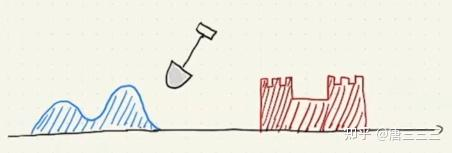
\includegraphics[width=0.8\textwidth]{png/SandMoving.jpg}
        \caption{The sand-moving problem.}
    \end{figure}

    \pause
    Let's denote the source shape by $f(x)$ and the target by $g(x)$. 
    The sand-moving problem cound be formulated as: 
    find a \textbf{transport mapping} $T:\R\to\R$ to minimize
    \begin{equation}
        \int_{\R} |T(x)-x|f(x)\;dx,
    \end{equation}
    which satisfies
    \begin{equation}
        \int_{T(U)} g(x)\;dx = \int_{U} f(x)\;dx\; \text{for all open interval}\; U\subset\R.
    \end{equation}
\end{frame}

\begin{frame}{The allocation problem}
    \footnotesize
    There are some steel coils to be transported from warehouses to factories.
    The transport cost is \$1 per coil and per kilometer.
    How to minimize the total cost?

    \begin{figure}
        \captionsetup{font=scriptsize}
        \centering
        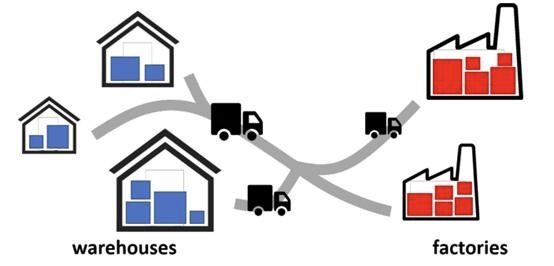
\includegraphics[width=0.6\textwidth]{png/SteelTransport.jpg}
        \caption{The allocation problem.}
    \end{figure}

    \pause\vspace{-.5em}
    Assume the $i$-th warehouse has $a_i$ coils and the $j$-th factory
    needs $b_i$ coils. And assume the distance between the $i$-th warehouse
    and the $j$-th factory is $d_{ij}$. The allocation problem could be 
    formulated as: find a \textbf{transport matrix} $v_{ij}$ to minimize
    \begin{equation}
        \sum_{i,j} d_{ij}v_{ij}
    \end{equation}
    which satisfies
    \begin{equation}
        a_i=\sum_{j} v_{ij},\quad \forall i,
        \qquad \text{and} \qquad 
        b_j=\sum_{i} v_{ij},\quad \forall j.
    \end{equation}
\end{frame}